\chapter{Geoid problem}\label{chap:content}

Geoid, in the field of geodynamics, represents the shape of a gravity equipotential across the whole of Earth's surface. Detailed maps of geoid elevation with contours spaced as close as 1m can show the effect of tectonic features such as deep sea trenches, outer arc rises, and oceanic ridges and troughs on the height of the geoid, which could provide powerful constraints that must be satisfied by the next generation of geodynamic models along with other data such as high quality determinations of surface deformation and new high resolution seismic data. \citep{10.1038_299104a0}

Geoid, as shown in the Figure \ref{figure:geoid_factors}, is generally related to both the 3D density field of the Earth and the radial viscosity profile of the Earth's mantle. However, a recent research shows that modelling that treats the geoid as being purely based on density variation near the surface can poorly explain the accurately observed geoid measurements with a satellite. \citep{10.1098_rsta.1989.0038}

Therefore, in this research, we aim to use Neural Network as a way to forward model the geoid problem,
assuming that viscosity varying in the radial direction with depth is the most important factor.

\begin{figure}[H]
    \centering
    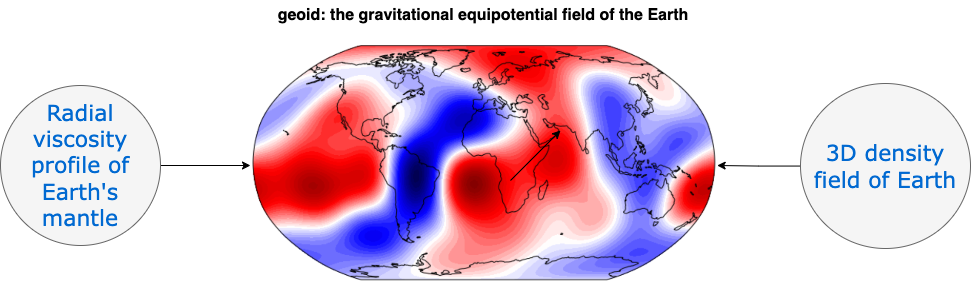
\includegraphics[scale=0.4]{figures/geoid_images/Geoid.png}
    \caption{Geoid and its two related factors.}
    \label{figure:geoid_factors}
\end{figure}

To explore the usage of Earth's viscosity to model the geoid using NNs, we use a 1D spherically symmetric viscosity model to compute a geoid surface in terms of some spherical harmonics coefficients that can be used to construct the geoid surface. To further simplify this problem, the dataset used for this research uses a reduced prior such that the perturbations to the output are smaller.


\section{Dataset of geoid prediction}

The reduced dataset consists of 1000 pairs of input and output. In the dataset, input is a vector with 257 values indicating a 1D spherically symmetric viscosity model and output is a vector with 60 values representing a set of spherical harmonic coefficients describing the geoid height on the surface of the Earth. Figure \ref{figure:geoid_sample} here is a sample geoid field constructed from a random set of 60 geoid coefficients from the output data, where the units of the geoid are in metres and represent values greater or less than some reference value.

\begin{figure}[H]
    \caption{Sample geoid field, where the units of the geoid are in metres and represent values greater or less than some reference value.}
    \label{figure:geoid_sample}
    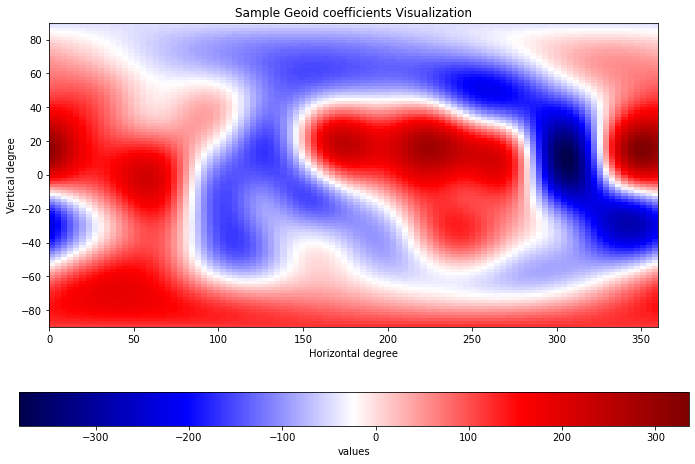
\includegraphics[scale=0.6]{figures/geoid_images/Geoid_Sample_visualization.png}
\end{figure}

To further observe the patterns in the input and the output, 10 pairs of input and output are plotted in Figure \ref{figure:geoid_input} and Figure \ref{figure:geoid_output}.

\begin{figure}[H]
    \centering
    \caption{Every 100th input in the dataset.}
    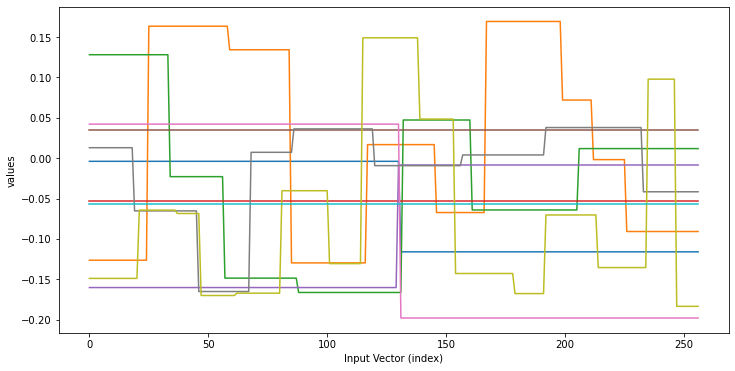
\includegraphics[scale=0.5]{figures/geoid_images/Geoid_sample_input.png}
    \label{figure:geoid_input}
\end{figure}

\begin{figure}[H]
    \centering
    \caption{Every 100th output in the dataset.}
    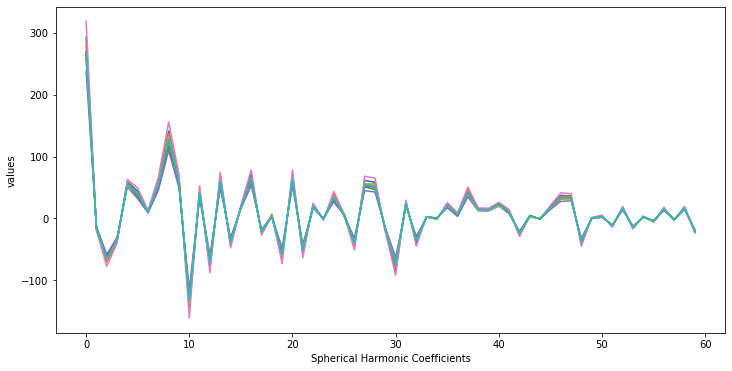
\includegraphics[scale=0.5]{figures/geoid_images/Geoid_sample_output.png}
    \label{figure:geoid_output}
\end{figure}

From the second plot we can observe that the outputs in the dataset can be seen as some "curves" with the same patterns but with different amplitude. In this case, each of the 60 coefficients in the output data are normalised to be between 0 and 1 using their maximum and minimum values separately before feeding into the neural network. This is because each of the parameters in an output vector can be seen as equally important and we want to prevent the neural network from spending most of its effort learning the parameter with a higher range of values. Hence, one can expect a higher accuracy when the parameters in the output data are standardized to the same range.

After the output data is normalised using a scalar, the entire dataset is randomly divided in a ratio of 8:1:1: 80 per cent of the dataset is used for training, 10 per cent of the data for testing accuracy and the remaining 10 per cent to perform validation during training and prevent overfitting. For a dataset with 1000 samples, this result in a train-test-validation split of 800-100-100.


\section{Fully Connected Neural Network for Prediction}

To test feed-forward fully connected neural network (FNN) with different architectures (e.g. different number of hidden layers and neurons per hidden layer) or other sets of hyperparameters (e.g. optimizer), a systematic testing method is applied. This method mainly consists of three files: one text file to store all the different set of FNN architectures and hyperparameters in a text format, one Jupyter Notebook file to fetch all these combinations of architectures and hyperparameters line by line, build them as FNN models and train these models, and another Jupyter Notebook file for testing and visualisation of the trained models by specifying the path of a trained model.

The trained FNN architecture (in the format of a light-weight file) along with another text file contains the training loss and validation loss during training will be stored in a specified path for further testing and visualisation. The name of these two files uniquely defines each experiment by including the values of hyperparameters used to generate this model in the file names. These files are also put in separate folders with the folder name associated with commit IDs to handle tracking of the process during the research in an educated or extensible way.

In this way, one can open the same Jupyter Notebook for testing in different browser tabs, and then visualize simultaneously different models in different tabs using a cell in which the paths to the FNN model and its training data are specified. 

The systematic testing capability is implemented here to ensure traceability. In other words, as different values of the hyperparameters are tested, We would like to be able to record the results (e.g., the trained network and the training data) so that we don't have to repeat them again or rely on our memory to compare the the performance of different structures.

Also, to prevent overfitting, a variation of the early-stopping method is used during training. The normal early-stopping method let the network train until the error function evaluated on the validation set starts to increase beyond a certain threshold \citep{10.1007_978-3-642-35289-8_5}, while my implementation only stores the best model during training (the one with the lowest validation loss) in a specified path and allows the network to keep training as normal. In this case, the output model is the best model instead of the last trained model. This method is also used in the upcoming chapters when implementing the ConvAE, FNN and LSTM to solve the mantle convection problem.

After testing with NNs with different number of hidden layers and neurons per hidden layer, we found that FNN with a total number 3–4 hidden layers seemed to perform the best.

In the following figures, we present results from a FNN with 4 hidden layers with 200, 160, 120 and 80 neurons, ReLU as activation function, MSELoss as loss function, and trained for 200 epochs using Mini-Batch Gradient Descent (with a batch size of 16).

One thing to notice is that the loss value, which is back-propagated during the training process, is calculated using the prediction and the normalised output. In this case, the best case and the worst case shown as below are also defined upon the value of this normalised error in order to be consistent, including the training loss and validation loss in Figure \ref{figure:geoid_losses}, the overall testing result in Figure \ref{figure:geoid_testing},  the most accurate geoid prediction in Figure \ref{figure:geoid_best} and the least accurate geoid prediction in Figure \ref{figure:geoid_worst}.

\begin{figure}[H]
    \caption{Training loss and Validation loss.}
    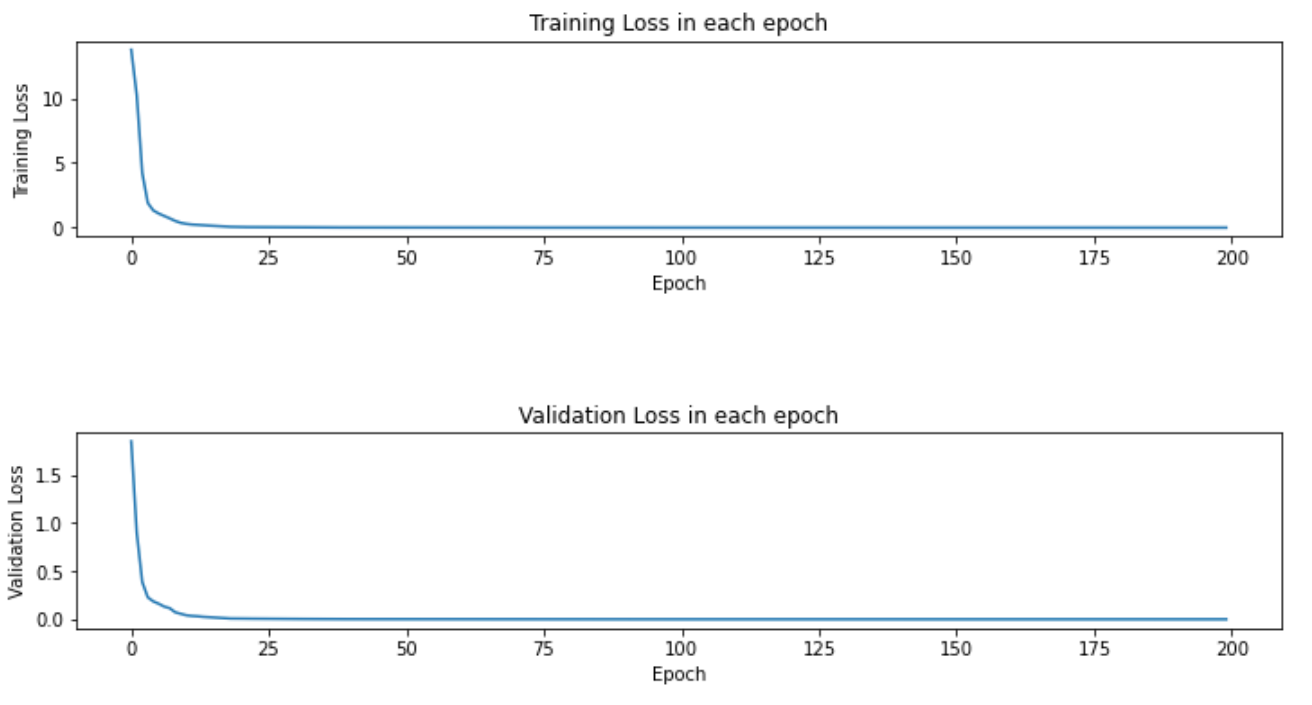
\includegraphics[scale=0.6]{figures/geoid_images/Geoid_trainingData.png}
    \label{figure:geoid_losses}
\end{figure}

\begin{figure}[H]
    \caption{Overall testing result.}
    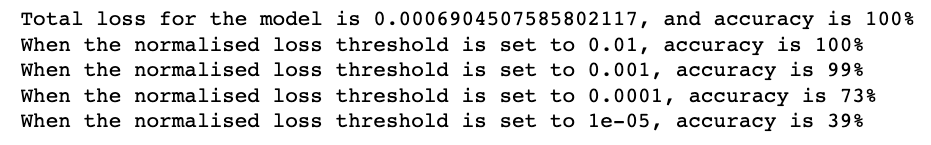
\includegraphics[scale=0.8]{figures/geoid_images/Geoid_OverallTesting.png}
    \label{figure:geoid_testing}
\end{figure}

\begin{figure}[H]
    \caption{Most accurate geoid prediction.}
    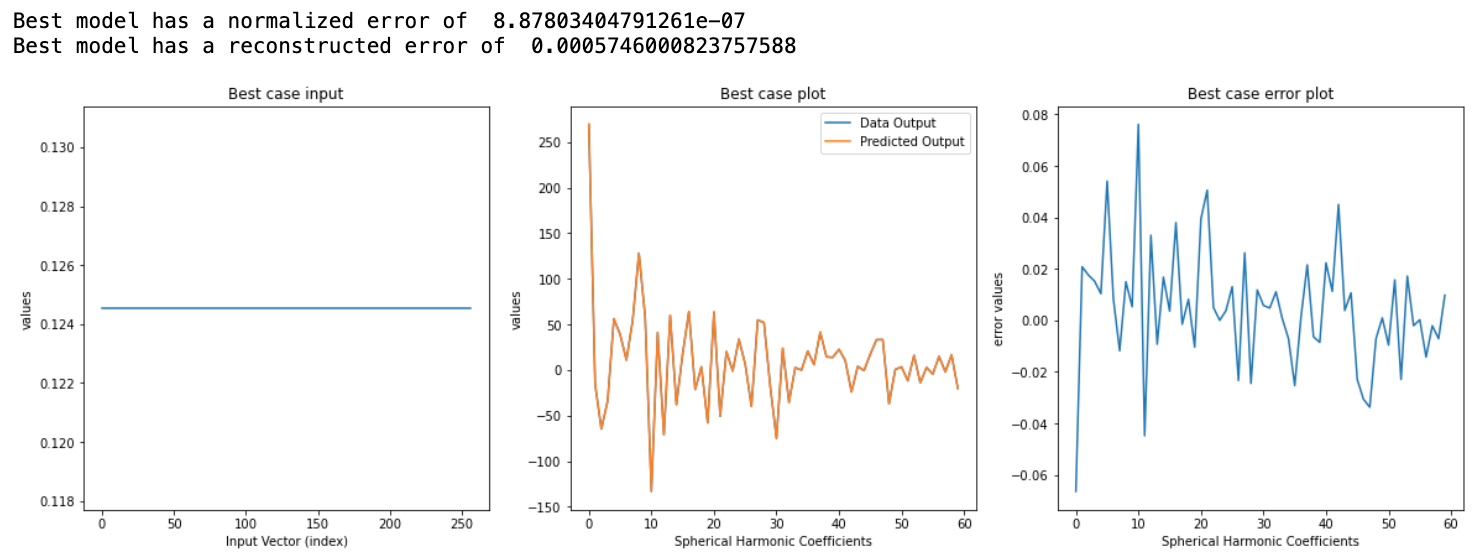
\includegraphics[scale=0.6]{figures/geoid_images/Geoid_Best.png}
    \label{figure:geoid_best}
\end{figure}

\begin{figure}[H]
    \caption{Least accurate geoid prediction.}
    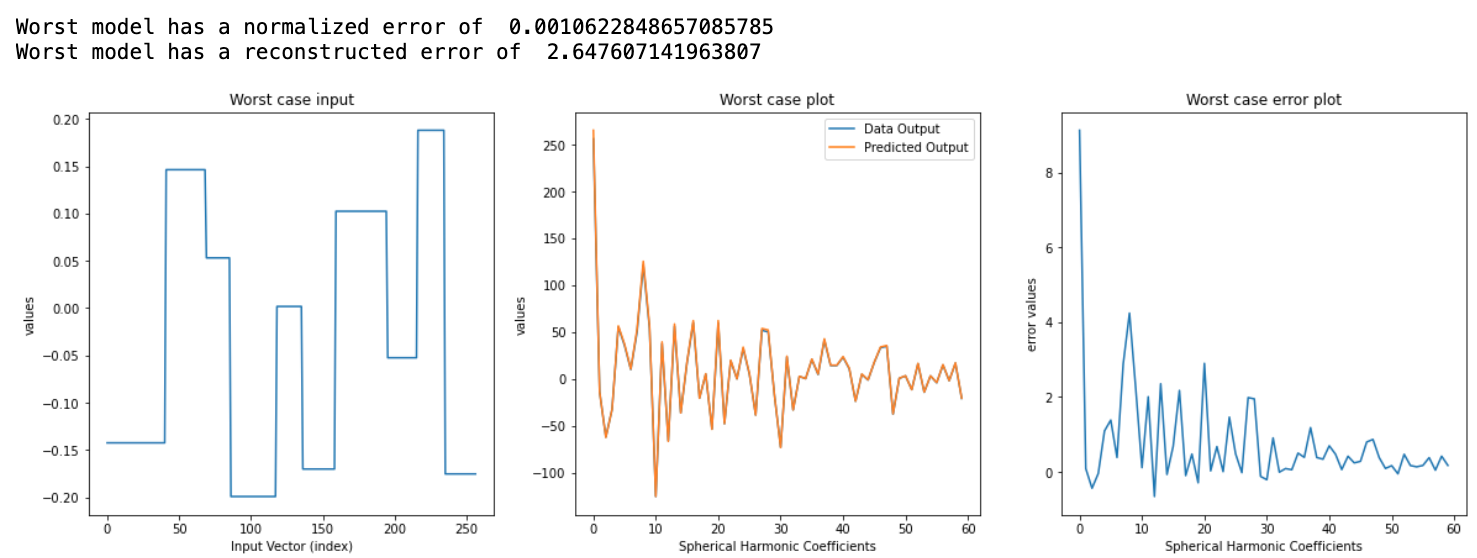
\includegraphics[scale=0.6]{figures/geoid_images/Geoid_Worst.png}
    \label{figure:geoid_worst}
\end{figure}

On average, both the normalised loss and the reconstructed loss are low and no overfitting occurs. The accuracy of the prediction is nearly 100\% when the threshold is set to be 10 times lower than the worst loss value. 

For further testings, the geoid fields constructed using the set of 60 coefficients produced by the FNN in both the best case and the worst case are visualized in Figure \ref{figure:geoid_best_visual} and Figure \ref{figure:geoid_worst_visual}, along with the fields produced by the ground truth and the error maps representing the difference between the prediction and the ground truth.

\begin{figure}[H]
    \caption{Visualization of the most accurate geoid prediction.}
    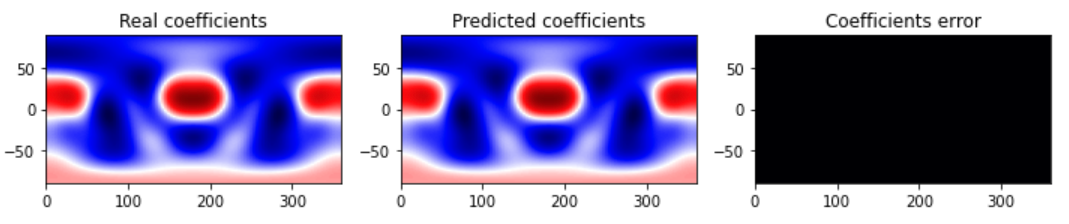
\includegraphics[scale=0.4]{figures/geoid_images/Geoid_Best_visualization.png}
    \label{figure:geoid_best_visual}
\end{figure}

\begin{figure}[H]
    \caption{Visualization of the least accurate geoid prediction.}
    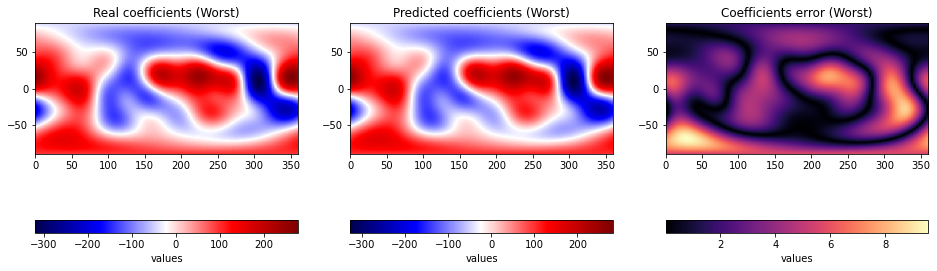
\includegraphics[scale=0.4]{figures/geoid_images/Geoid_Worst_visualization.png}
    \label{figure:geoid_worst_visual}
\end{figure}

We can observe that the result produced by the FNN is in high quality even in the worst case, where the maximum error between the real geoid field and the predicted geoid field is about 60 times less than the range of real values. The real geoid field and the predicted field also have the same patterns in both cases, meaning that FNN is able to capture the characteristic of the data in its prediction.

Overall, we constructed a systematic framework for rapidly testing different FNN architectures in a reproducible way, and we were able to create a highly accurate FNN as a surrogate forward model for the geoid problem, this could be used in further research in inverse problems involving observations of the Earths geoid.